\documentclass[a4paper]{article}
\usepackage{graphicx}
\graphicspath{{./figures/}}
\usepackage[italian]{babel}
\usepackage{float}
\usepackage{amsmath, amssymb, braket}
\usepackage{listings}
\usepackage{tikz}
\usetikzlibrary{shapes, arrows, automata, petri, decorations.markings, decorations.pathreplacing, positioning, calc}

\usepackage{hyperref}
\hypersetup{
    colorlinks=false,
}

% Code blocks
\definecolor{codegreen}{rgb}{0,0.6,0}
\definecolor{codegray}{rgb}{0.5,0.5,0.5}
\definecolor{codepurple}{rgb}{0.58,0,0.82}
\definecolor{backcolour}{rgb}{0.95,0.95,0.95}

\lstdefinestyle{mystyle}{
	backgroundcolor=\color{backcolour},
	commentstyle=\color{codegreen},
	keywordstyle=\color{magenta},
	numberstyle=\tiny\color{codegray},
	stringstyle=\color{codepurple},
	basicstyle=\ttfamily\footnotesize,
	breakatwhitespace=false,
	breaklines=true,
	captionpos=b,
	keepspaces=true,
	numbers=left,
	numbersep=5pt,
	showspaces=false,
	showstringspaces=false,
	showtabs=false,
	tabsize=2
}

\lstset{style=mystyle}

\begin{document}

% Title ------------------------------------------------------------------------------
\title{Introduzione alla meccanica quantistica per il quantum computing\\[1ex]
\large Quantum Key Distribution - Protocollo BB84
}

\author{
\vspace{0.8cm}
Università di Verona\\
Imbriani Paolo - VR500437\\
Irimie Fabio - VR501504\\[8ex]
Profssa. Daffara Claudia
}

\begin{figure}
    \centering
    
\includegraphics[width=0.3\textwidth]{UniversityofVerona.png}
\end{figure}

\maketitle 

\pagebreak
% Title ------------------------------------------------------------------------------

\tableofcontents

\pagebreak

\section{Introduzione}
Fabio e Paolo vogliono instaurare un canale di comunicazione sicuro, in modo da poter
inviare messaggi privati senza che un eventuale attaccante possa intercettarli.
I due si affidano alla crittografia, che permette di codificare i messaggi in modo che
solo il destinatario possa decifrarli.

I due potrebbero utilizzare un metodo classico, come ad esempio il cifrario di Cesare che
prevede di sostituire ogni lettera con una lettera che si trova un certo numero di posizioni
più avanti nell'alfabeto. Ad esempio:
\[
\begin{aligned}
    \text{A} & \rightarrow \text{D} \\
    \text{B} & \rightarrow \text{E} \\
    \text{C} & \rightarrow \text{F} \\
             & \hspace{0.5em}\vdots \\
    \text{Z} & \rightarrow \text{C}
\end{aligned}
\] 
Immaginiamo che Fabio voglia inviare un messaggio a Paolo, per far sì che Paolo
possa decifrare il messaggio, Fabio deve comunicargli la chiave, ovvero il numero
di posizioni da spostare nell'alfabeto. Questo metodo è facilmente intercettabile,
infatti l'attaccante può semplicemente provare tutte le possibili chiavi fino a trovare
quella giusta. Questo tipo di crittografia è detta simmetrica, in quanto sia il mittente
che il destinatario devono possedere la chiave per cifrare e decifrare il messaggio.

\section{Cos'è BB84?}
Per far sì che Fabio e Paolo possano creare un canale di comunicazione sicuro, devono
trovare un modo per scambiarsi la chiave in segreto. Però anche in questo caso, la 
condivisione della chiave deve essere fatta in un canale sicuro, che è il problema
che vogliamo risolvere dal principio!

Il protocollo BB84 è un protocollo di \textit{Quantum Key Distribution} che risolve questo
problema. Se Fabio usasse questo protocollo per trasmettere la chiave a Paolo, loro
potrebbero sapere con \textit{quasi} assoluta certezza se la chiave è stata intercettata o
meno.
\begin{itemize}
  \item Se la chiave \textbf{non} è stata intercettata, Fabio e Paolo avrebbero una chiave
    segreta per instaurare un canale di comunicazione sicuro.

  \item Se la chiave \textbf{è} stata intercettata, Fabio e Paolo possono decidere di non
    utilizzare la chiave e di ripetere il protocollo.
\end{itemize}

\subsection{Requisiti}
Per funzionare, il protocollo BB84 ha bisogno dei seguenti requisiti:
\begin{itemize}
  \item Sia Fabio che Paolo devono avere accesso al proprio computer quantistico.

  \item Devono avere un canale di trasmissione capace di trasmettere qubit. Questo
    potrebbe essere qualche tipo di cavo a fibra ottica capace di trasmettere fotoni
    polarizzati.

  \item Devono avere un canale di comunicazione classico. Siccome è impossibile
    assicurare una sicurezza perfetta, bisogna assumere che qualsiasi canale classico
    può essere intercettato.
\end{itemize}

\subsection{Funzionamento}
I passaggi del protocollo sono i seguenti:
\begin{enumerate}
  \item Fabio crea una stringa casuale di bit, e per ogni bit, lui sceglie casualmente
    una base in cui codificarlo.

  \item Fabio codifica i bit in qubit usando la base scelta, e invia i qubit al computer
    quantistico di Paolo attraverso un canale di comunicazione quantistico.

  \item Anche Paolo sceglie casualmente una base secondo cui decodificare ogni qubit
    ricevuto. Quindi misura ogni qubit nella base che ha scelto.

  \item Fabio utilizza un canale di comunicazione classico per dire a Paolo che basi
    ha scelto per la codifica. Poi comunica anche i primi bit della chiave non codificati.

  \item Paolo analizza questi primi bit per determinare se un intercettatore\\
    (Amos) è riuscito ad entrare nel canale di comunicazione quantistico e intercettare i
    qubit che Fabio gli ha inviato.

  \item Si distinguono due casi:
    \begin{itemize}
    \item Se Amos \textbf{non} ha intercettato i qubit, Fabio e Paolo possono considerare
      tutti i qubit che hanno scelto \textbf{in comune}, cioè con la stessa base, come
      la loro chiave segreta.

    \item Se Amos \textbf{ha} intercettato i qubit, Fabio e Paolo devono ripetere il
      processo da capo.
  \end{itemize}
\end{enumerate}

\section{Scenario concreto}
Prendiamo in considerazione un esempio concreto per capire meglio il protocollo BB84,
in cui Fabio è il mittente e Paolo è il destinatario. Questo esempio è scritto in Python
e utilizza la libreria \texttt{qiskit} per simulare il computer quantistico. Le librerie
da importare sono le seguenti:
\begin{lstlisting}[language=Python]
from qiskit import *
import random
\end{lstlisting}

\subsection{Codifica}
Per prima cosa Fabio deve scegliere una sequenza di bit e basi da utilizzare per
codificare i bit in qubit. Un qubit può essere rappresentato come un vettore sulla sfera
di Bloch, che è una rappresentazione geometrica di uno stato quantistico. Ogni asse
può essere considerato come una possibile base. Quindi se un vettore punta in alto, il
qubit è codificato in $\ket{0}$, se punta in basso è codificato in $\ket{1}$. L'asse
verticale è chiamato \textit{asse \( Z \)}. Nella base \( Z \) possiamo codificare 
lo 0 come $\ket{0}$ (figura \ref{fig:base_z} a sinistra) e l'1 come $\ket{1}$
(figura \ref{fig:base_z} a destra).
\begin{figure}[H]
  \centering
  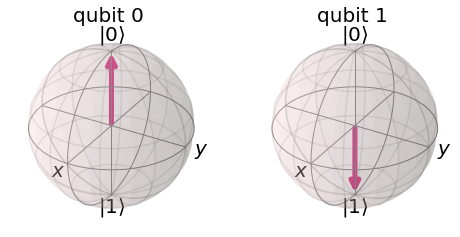
\includegraphics[width=0.6\textwidth]{base_z}
  \caption{Base Z}\label{fig:base_z}
\end{figure}
Un altro modo di codificare i qubit è utilizzare la base \( X \), in cui lo 0 è
rappresentato da $\ket{+}$ (figura \ref{fig:base_x} a sinistra) e l'1 da $\ket{-}$
(figura \ref{fig:base_x} a destra).
\begin{figure}[H]
  \centering
  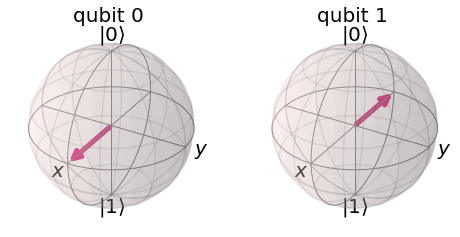
\includegraphics[width=0.6\textwidth]{base_x}
  \caption{Base X}\label{fig:base_x}
\end{figure}

Il primo passo per Fabio è generare casualmente una stringa di bit di lunghezza
arbitraria, ad esempio 300 bit.
\begin{lstlisting}[language=Python]
KEY_LENGTH = 300 # Lunghezza della chiave
random.seed(0)

# Genera una chiave casuale di lunghezza KEY_LENGTH
fabio_bits = ""
for i in range(KEY_LENGTH):
    randBit = random.randint(0, 1) # Numero casuale 0 o 1
    fabio_bits += str(randBit) # Aggiungi il bit alla chiave
    
print("I bit che Fabio invia sono: " + fabio_bits[:10] + "...")
\end{lstlisting}
\begin{lstlisting}
I bit che Fabio invia sono: 1011101010...
\end{lstlisting}
Successivamente Fabio sceglie una base per ogni bit (o in base \( Z \) o in base \( X \)).
\begin{lstlisting}[language=Python]
def generate_random_bases(num_of_bases):
    """Questa funzione seleziona una base casuale per ogni bit"""
    bases_string = ""
    for i in range(num_of_bases):
        randBasis = random.randint(0, 1)

        if randBasis == 0:
            bases_string += "Z" 
        else:
            bases_string += "X"
            
    return bases_string

# Fabio sceglie casualmente una base per ogni bit
fabio_bases = generate_random_bases(KEY_LENGTH)
print("Le basi che Fabio usa sono: " + fabio_bases[:10] + "...")
\end{lstlisting}
\begin{lstlisting}
Le basi che Fabio usa sono: XXZZZXZXZZ...
\end{lstlisting}
Ora Fabio, sul suo computer quantistico, codifica i bit in qubit utilizzando le basi
che ha scelto, creando così una stringa di 300 qubit. Successivamente, Fabio invia i
qubit al computer quantistico di Paolo attraverso un canale di comunicazione
quantistico.

Di default, Qiskit utilizza la base \( Z \) per codificare i qubit e tutti i qubit sono
inizializzati in $\ket{0}$. Per trasformare il qubit in $\ket{1}$ bisogna applicare
una porta \( X \).

Mentre invece, per codificare i qubit in base \( X \) si inizia con i corrispondenti
$\ket{0}$ e $\ket{1}$ e si applica una porta \( H \) (Hadamard) per trasformarli rispettivamente
in $\ket{+}$ e $\ket{-}$.

La tabella delle conversioni è la seguente:
\begin{table}[H]
  \centering
  \begin{tabular}{|c|c|c|c|}
    \hline
    \textbf{Bit} & \textbf{Base} & \textbf{Stato} & \textbf{Porta} \\ \hline
    0 & Z & $\ket{0}$ & - \\ \hline
    1 & Z & $\ket{1}$ & \( X \) \\ \hline
    0 & X & $\ket{+}$ & \( H \) \\ \hline
    1 & X & $\ket{-}$ & \( H,X \) \\ \hline
  \end{tabular}
\end{table}
Usando come riferimento questa tabella, il circuito quantistico per codificare i bit
in qubit è il seguente:
\begin{lstlisting}[language=Python]
def encode(bits, bases):
    """La funzione codifica ogni bit nella base data"""
    
    encoded_qubits = []
    
    for bit, basis in zip(bits, bases):
        # Crea un circuito quantistico per ogni qubit
        qc = QuantumCircuit(1, 1)
        
        # Casi possibili
        if bit=="0" and basis == "Z":
            encoded_qubits.append(qc) # Non serve applicare nessuna porta

        elif bit=="1" and basis == "Z":
            qc.x(0) # Applica porta X
            encoded_qubits.append(qc)

        elif bit=="0" and basis == "X":
            qc.h(0) # Applica porta H
            encoded_qubits.append(qc)

        elif bit=="1" and basis == "X":
            qc.x(0) # Applica porta X
            qc.h(0) # Applica porta H
            encoded_qubits.append(qc)
            
    return (encoded_qubits)


# Codifica i bit di Fabio
encoded_qubits = encode(fabio_bits, alice_bases)

# Print circuits for first 5 qubits.
for i in range(5):
    print(encoded_qubits[i])
print("etc.")
\end{lstlisting}

\subsection{Trasmissione}
    
\end{document}
